\renewcommand\TheFile{weekplan.tex}
\SVN $Author: hom $
\SVN $Revision: 126 $
\SVN $Id: weekplan.tex 126 2017-10-24 07:34:14Z hom $
\SVN $Date: 2017-10-24 09:34:14 +0200 (Tue, 24 Oct 2017) $
\SVN $State: Exp $
\begin{savequote}[8cm]
  \sffamily
  Genius is one percent inspiration and ninety-nine percent perspiration.
  \qauthor{Thomas A. Edison}
\end{savequote}
\chapter{Execution of the project}

\parpic(51mm,39mm){
\includegraphics[width=51mm]{figures/WorkinProgress.jpg}}The
main focus of this project is on reactive systems and usage of
design patterns. This explains why we enforce a rather strict plan, to
make sure that all goals are met and groups do not get into trouble
due to inadequate planning. Note that the planing is quite tight. So
not only work as a team towards the next delivery (there is one every
week), but properly use all available manpower. That is: Near a
delivery deadline most of your team members should be done with the
work for that deadline and 2 project members are  involved in preparing
the demo for the deadline. The others should be working on
investigating the deliverables for the next deadline.

\section{Products}

The products of this assignment are:
\begin{enumerate}
\item Report
\item Model
\item Implementation
\end{enumerate}

\subsection{How to deliver your assignment products}
All electronic products must be handed in via \href{https://peerweb.fontysvenlo.org/}{peerweb}. See peerweb for all deadlines.
\begin{enumerate}
\item Report: one document describing your analysis, design and its
  implementation, test installation and user manual to be handed in on
  paper too, \emph{properly bound at the copy shop}. The document should also
  contain a reference to the repository. 
  See the weekly plan for what the document should contain. The
  design diagrams, user interface illustrations etc. are copied into
  and explained in the report document. In the document code fragments
  are shown only when relevant. E.g.  when the implementation is
  discussed in the describing text.
\item  Models: One model file in the Visual Paradigm UML tool.
  The models should contain analysis, design and implementation as
  well as a reverse engineered model of the complete
  implementation. For practical reasons you may use more then one
  model file for each of the phases analysis, design and
  implementation. You may hand in three distinct models.
\item Implementation: All (re)sources needed to build the project
  should be in the project repository at all times. The sources should
  be accompanied with an ant build script. Most of the time the
  Netbeans build.xml script will do.
  
  For all but the first week you should produce a executable artefact
  or runnable program. 
  By checking out the project and calling ant jar should result in a
  functional and runnable jar file. Say the produced jar file is
  called \Okis{dist/SuperElevator.jar}
  I will use the file like this:\\
  \frame{\scriptsize\Code{java~-cp~dist/SuperElevator.jar~nl.fontys.sevenlo.prj32.DemoWeekX}}.
  
  The prefix \Code{nl.fontys.sevenlo.prj32} is mandatory for all your
  packages. You may (maybe should) have additional packages under this
  top package name. You may also create several Netbeans projects with
  additional package and directory structures to reflect your
  functional decomposition.
  
  Each week that has an executable will have a Main class named\\
  \Code{nl.fontys.sevenlo.prj32.DemoWeek\textit{\textbf{weeknr}}}. For each
  week, except the first, there will be a hand in of a runnable jar file.
\end{enumerate}

\section{Naming conventions}
\paragraph{Libraries}
You will be using supplied libraries for the control of the
hardware. You may look at it as a layered architecture. The hardware
layer is provided by the \Code{IOWarrior} Library. It is provided by
the manufacturer of the IOWarrior chip, Code Mercenaries GmbH.

The bit io abstraction layer is provided by \Okis{sevenlohwio}
library. It provides a bit wise io abstraction.

The \Okis{sevenlowarrior} combines the facilities provided by the
hardware with the abstraction layer and thus provides USB based
bitwise io. 

For testing purposes in a gui environment sevenlowarrior uses the
\Okis{sevenlowidgets} library. Aside the use for iowarrior testing it
also provides some goodies that can be use full in your elevator
implementation.

The widgets library itself uses some resources that must be loaded
from the class path. We use \Okis{sevenloutils} for that.

To be able to use these libraries in a platform and java/netbeans installation
independent way, create netbeans libraries.


You get most comfort if you install the libraries complete with source
and javadoc. 

Since 2017, the libraries are built as maven projects. Since April 2019, all sources have moved
to github at \href{https://github.com/sebivenlo/sevenloio}{SEVenloio at Github}

A maven repository is maintained at \url{https://www.fontysvenlo.org/repository}, which
you can easily add to your private maven settings by adding said repository to your mavenconfig in the \texttt{\~/.m2/settings.xml} file.
Make sure your also activate that profile.

\begin{lstlisting}[language=xml,caption={settings}]
<profile>
  <id>sebivenlo</id>
  <repositories>
    <repository>
       <id>fontysvenlo.org</id>
       <url>https://www.fontysvenlo.org/repository</url>
    </repository>
  </repositories>
</profile>
\end{lstlisting}


Activation can be done as follows in the same settings.xml file:

\begin{lstlisting}[language=xml,caption={activate profile}]
  <activeProfiles>
     <activeProfile>sebivenlo</activeProfile>
  </activeProfiles>
\end{lstlisting}

The libraries you might want to include in your respository are mentioned in the maven coordinates below:

\begin{lstlisting}[language=xml,caption={All sebivenlo io stuff. Add/adapt version numbers before use.}]
  <dependency>
     <groupId>nl.fontys.sevenlo</groupId>
     <artifactId>sevenloutils</artifactId>
     <version>1.2</version>
  </dependency>
  <dependency>
     <groupId>nl.fontys.sevenlo</groupId>
     <artifactId>sevenlohwio</artifactId>
     <version>3.2.2</version>
  </dependency>
  <dependency>
     <groupId>nl.fontys.sevenlo</groupId>
     <artifactId>sevenlonetio</artifactId>
     <version>1.0-SNAPSHOT</version>
  </dependency>
  <dependency>
     <groupId>nl.fontys.sevenlo</groupId>
     <artifactId>sevenlowarrior</artifactId>
     <version>1.7.2</version>
  </dependency>
  <dependency>
     <groupId>nl.fontys.sevenlo</groupId>
     <artifactId>sevenlowidgets</artifactId>
     <version>1.1</version>
  </dependency>
\end{lstlisting}


In the git hub repository you canb also find some demo and sample code to get you started.





%       The names of these libraries and the installation\footnote{The paths
%   used are for Debian/Ubuntu Linux.} steps as netbeans library are:
% {
% \setlength\parsep{0pt}
% \setlength\topsep{0pt}
% \setlength\partopsep{0pt}
% \setlength\parskip{0pt}
% \setlength\itemsep{0pt}
% \newcommand\Classpath{[Classpath]}
% \newcommand\Sources{[Source]}
% \newcommand\Javadoc{[Javadoc]}
% \begin{description}
% \item[CodeMercenaries] The hardware access layer.
%   \begin{description}
%   \item[\Classpath] The library proper is at \Code{/usr/share/java/codemercs.jar}.
%   \item[\Sources] Add the file \Code{/usr/share/java/codemercs-src.jar}.
%   \item[\Javadoc] Add the file \Code{/usr/share/java/codemercs-doc.zip}.
%   \end{description}
% \item[SEVenloHWIO] The bit io abstraction layer. 
%   \begin{description}
%   \item[\Classpath] The library proper is at \Code{/usr/share/java/sevenlohwio.jar}.
%   \item[\Sources] Add the file \Code{/usr/share/java/sevenlohwio-src.jar}.
%   \item[\Javadoc] Add the file \Code{/usr/share/java/sevenlohwio-doc.zip}.
%   \end{description}
% \item[SEVenloWarrior] The bit io abstraction layer. 
%   \begin{description}
%   \item[\Classpath] The library proper is at \Code{/usr/share/java/sevenlowarrior.jar}.
%   \item[\Sources] Add the file \Code{/usr/share/java/sevenlowarrior-src.jar}.
%   \item[\Javadoc] Add the file \Code{/usr/share/java/sevenlowarrior-doc.zip}.
%   \end{description}
% \item[SEVenloWidgets] The gui widgets. 
%   \begin{description}
%   \item[\Classpath] The library proper is at \Code{/usr/share/java/sevenlowidgets.jar}.
%   \item[\Sources] Add the file \Code{/usr/share/java/sevenlowidgets-src.jar}.
%   \item[\Javadoc] Add the file \Code{/usr/share/java/sevenlowidgets-doc.zip}.
%   \end{description}
% \item[SEVenloUtils] The resource utils. 
%   \begin{description}
%   \item[\Classpath] The library proper is at \Code{/usr/share/java/sevenloutils.jar}.
%   \item[\Sources] Add the file \Code{/usr/share/java/sevenloutils-src.jar}.
%   \item[\Javadoc] Add the file \Code{/usr/share/java/sevenloutils-doc.zip}.
%   \end{description}
% \end{description}
% } % end of lengths
% All these libraries can be found at the module website.

% To ease your getting into the matter, we've created a project in GIT,
% containing a sub directory containing a maven netbeans project, called
% bitfactoryexample. You can clone it with the coordinates
% \texttt{git@fontysvenlo.org:2013/prj32m1/g4}. You should be able to
%   build and run this project. The command line way to build it is
% \texttt{mvn compile assembly:single}, which will build a singe jar
% containing all the required libraries. This maven command should pull
% in all the required resources and libraries.

% If you also would like to get the sevenlo libraries described
% above. Clone the repository \texttt{git@fontysvenlo.org:2013/prj32m1/g4}.



\subsection{Group repository}
\parpic[rs]{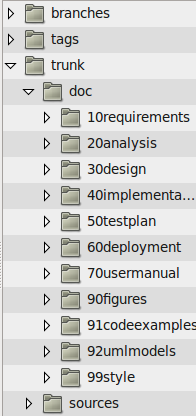
\includegraphics[width=39mm]{figures/projecttree.png}}The
repository contains a predefined directory structure. All source 
code (including tests) should be placed under \Code{sources}. The \Code{doc}
directory is intended for the documentation including the analysis and
design models. Use Visual Paradigm for your UML modelling. It also
integrates quite well with subversion\footnote{with git I do not know} through its \textit{team work}
capabilities. The doc directory strongly hints at preparing your
report using \LaTeX.

\paragraph{Project name} The netbeans projects shall be named with a
group prefix in front of them in the form of \Okis{gx\_}, where \textit{x} is
one of 01\ldots04  as in \Code{g01\_elevator}.

This also applies if you split your whole project into several
(netbeans) sub-projects for instance for specific subsystems. This is
a good idea anyway. So you might have a \Code{g01\_guiwidgets} library
project.

At the end you will have to deliver the complete deployable binary in
a zip file. This zip file will have the name gx\_elevator.zip. This
zip file must contain all that is needed to deploy the applications
via web start, using the jnlp protocol. The zip file should contain all
that is packed into the \Code{dist} subdirectory, including the dist
subdir itself. In \Linux that would be the \\
\framebox{\Code{zip -r g01\_elevator.zip dist}}\\
-command.

Tagging and branching of the documentation (doc) subtree is not required.
However the sources subtree will be tagged each week (see below).

A tag (and a branch) are simple copy commands in subversion. See the
appropriate documentation in the svnbook at
\url{http://svnbook.red-bean.com/nightly/en/index.html}. Use
the appropriate source and destination urls and all is done on the
server with minimal delay. Being versed at the subversion command line
is very rewarding here. If not sure, try things first in your
personal scratch pad repository.

In git, tagging is simple too, See \url{https://git-scm.com/book/en/v2/Git-Basics-Tagging}.

\paragraph{Tags} Each week the tutors will make a TAG with the name
pattern TAG\_WEEKx. Other TAGS may be used freely.

\paragraph{Branches} You develop on the trunk, which is where the most
project members are working. Near a deadline, some will be preparing
for the demo of that period. Consider using a branch for the last
preparations so that work by others does not inter fear with your demo
project. From there pick up the stuff from the trunk in a controlled
way by applying the proper \Okis{merge} commands from trunk.
Consider branch names like \Okis{LOGIC\_RELEASE} etc.

In Git you do not need branches for a local experiment, as long as you
do not push the incomplete experiment results to the origin.

\paragraph{Final delivery} The final deliveries are: reports in pdf file format and a java
jar containing all dependencies.


\section{Weekly planning}
The weekly rhythm must be strictly observed. The hand in for all but
the last deliverable will all be done using subversion to the URL
for your group as mentioned on the PRJ32 website. As hand in time the
svn time is taken. Note that this always is UTC, thus not the same as
your wall clock time.

During all project weeks you will keep a time record of all
the time spent on the project.

At the end of each project week the tutor will tag the repository with
a read only tag for all groups. The material in the tag is considered
handed in. The rest is not.

\setlength\extrarowheight{4pt}
\begin{longtable}{|p{10mm}|p{20mm}|p{90mm}|}%
  \caption{Week plan}\\\hline%
  \rowcolor[gray]{0.8}\textbf{week}&\textbf{delivery}&\textbf{Task and
    product}\\\hline%
 \endhead%
  \hline \multicolumn{3}{r}{\emph{week plan continued on next page}} 
 \endfoot%
  \hline \multicolumn{3}{c}{\textbf{End of week plan}}%
 \endlastfoot%

  1 & \begin{minipage}{18mm}
    SCM \\ TAG~WEEK1 
  \end{minipage}
  &  \begin{minipage}{90mm}
    \RaggedRight
    \vspace*{3mm}
    {\large\textbf{Analysis}}
    \begin{description}
    \item[Use case description] describing the main success
    scenarios (including the alarm scenario). (Hint: subdivide the
    journey into 4 sub scenarios; there is also an alarm scenario). 
  \item[Use case diagrams] showing the relations between the use cases.
  \item[Analysis class diagram] including CRC descriptions of the
    classes
  \item[Sequence diagrams] of the main scenarios. If you followed the
    advice in the use cases you should have 5 sequence diagrams.
  \item[State model] The system obviously has state behaviour. Model
    this state behaviour of the system and its subsystems using  state
    diagrams.
  \item[Data model] Data model is a posh\footnote{Posh is the not so posh word for chique} word for how to keep track of
    all requests and commands of the elevator system. Design a data
    model with appropriate operations. The data model may keep up and
    down requests separate from target requests. From the start think
    of multiple shaft systems.
    \end{description}
    
  \end{minipage}\\\hline
  2 & 
  \begin{minipage}{18mm}
    SCM\\ TAG~WEEK2
  \end{minipage}
  & \begin{minipage}{90mm}
    \RaggedRight
    \vspace*{3mm}
    {\large\textbf{Hardware subsystem and Data model}}
    Analysis, design and implementation of the hardware IO
    subsystem. The hardware elevator will be connected using USB and a
    small IOWarrior printed circuit board. You will be given the complete
    IOWarrior library (which is available from code mercenaries) plus a
    library that provides the elementary read and write operations to the
    hardware.
    
    Deliverables:
    \begin{description}
    \item[Class model IO subsystem] A complete design class model of the
      system. For the report you will need diagrams of the subsystems.
    \item[Implementation of IO subsystem] As usual: no implementation is
      complete without tests.
    \item[Data model and implementation] including tests of all the
    operations.
    The test on the data model \textbf{must} have 100\% statement
    coverage, to be determined with the Emma coverage plug in.
    \end{description}
  \end{minipage}
  \\\hline
  3 & \begin{minipage}{18mm}
    SCM\\  TAG~WEEK3
  \end{minipage}
  & \begin{minipage}{90mm}
    \RaggedRight
    \vspace*{3mm}
    {\large\textbf{GUI and simulation}} design and design and
    implementation of the widgets used in this design.
    
    Deliverables:
    \begin{description}
    \item[Drawing of the gui design] I would use inkscape. You might
      want to opt for Adobe Illustrator or a similar tool. Make sure
      you are able to deliver a vector type file. (SVG or PDF).
    \item[Widgets] The \textbf{Cage} which should provide obstruction detection
      functionality. \textbf{Up} and \textbf{down} buttons including
      the appropriate. \textbf{Floor sensor indicators} which show
      when a floor sensor is activated. 
      \textit{ButtonModels}. Target buttons. Note that all these
      widgets get rather little real estate in the GUI picture.
    \item[State machine](s) implementation  for the behaviour of the system. 
    \end{description}
    
  \end{minipage}
  \\\hline
  4 & \begin{minipage}{18mm}
    SCM\\TAG~WEEK4
  \end{minipage}
  & \begin{minipage}{90mm}
    \RaggedRight
    \vspace*{3mm}
  {\large\textbf{Data model and  GUI  integration}}
  
  Deliverables:
  \begin{description}
  \item[Integrated GUI simulation] that shows the functionality
    of the widgets and the whole system so far. This simulation
    should already behave like a normal elevator system with
    respect to state behaviour. The data model should be used.
  \item[Strategy design] Use the Strategy pattern to implement
    different behaviours of the system in several modes. Implement
    one simple but useful strategy.
    
    \end{description}    
  \end{minipage}
  \\\hline
  5 & \begin{minipage}{18mm}SCM \\TAG~WEEK5
  \end{minipage}
  & \begin{minipage}{90mm}
    \RaggedRight
    \vspace*{3mm}
    {\large\textbf{GUI - hardware integration}} with simple strategy.
    \begin{description}
    \item[Combined hardware and software model] in which the GUI shows
      two cages, one simulation and the other as a monitor to the
      hardware model. This implementation must be working for a
      building with 4 floors.
    \end{description}
    \vspace{.3\baselineskip}
  \end{minipage}
\\\hline
  6 & SCM TAG~WEEK6 & \begin{minipage}{90mm}
    \RaggedRight
    \vspace*{3mm}
    {\large\textbf{Additional strategy implementations}}
    \begin{description}
    \item[Strategy] implementations for the remaining operating modes.
    \end{description}
    {\large\textbf{Documenting, presentation and demo preparation}}
    \begin{description}
    \item[Complete class documentation] extract-able with javadoc.
    \item[all diagrams] for the report.
    \item[Report] with sections \textbf{requirements},
      \textbf{analysis}, \textbf{design}, \textbf{implementation
        details}, \textbf{test plan} describing what you intended to
      test, \textbf{deployment manual} and a \textbf{User manual}.
    \end{description}
    \vspace{.3\baselineskip}
  \end{minipage}
\\\hline
  7 & \begin{minipage}[b]{18mm}
    SCM + peerweb\\TAG~WEEK7\\
    +reports (.pdf) \\
    in peerweb
    \\
    presentation \\and\\ demo
  \end{minipage}
  & \begin{minipage}{90mm}
    \RaggedRight
    \vspace*{3mm}
    {\large\textbf{Delivery week}} in which the products are
    presented and demonstrated. During this demonstration the use of
    compilers, editors and the like is forbidden. All code should be
    runnable in delivered binary form. For Java that would be a jar
    file, possibly combined with a startup script. You may use several
    startup scripts to show different features of your application,
    but all  should use the same (set of) jar file(s).

    All groups will provide a zip file that contains an application
    that is deployable through a web site using Java web start. This
    zip file must be self contained and have no external dependencies
    that have to be pre-installed. This should provide  us to have
    very nice set of demo applications. See the netbeans documentation
    on how to do that. This application should be able to work with
    and without the iowarrior drivers and libraries installed. 

    All students must attend the presentation demonstration of all
    groups.

    \begin{description}
    \item[Final execution report] Time usage sheets for all group
      members summarised over the whole project. 
    \item[Defects report] Defects found during tests and integration
      with an impact analysis. An impact analysis describes what the
      subsequent effect of this defect is on the rest of or the
      overall system .
    \end{description}
  \end{minipage}
  \\\hline
\end{longtable}  
